\documentclass{article}
\usepackage[utf8]{inputenc}
\usepackage{multicol}
\usepackage{graphicx}
\graphicspath{{images/}}
\usepackage{subcaption}

\title{Computer Vision Coursework}
\author{Candidate number 167083}

\begin{document}

\setcounter{page}{0}
\maketitle\newpage


\section{Introduction}
In this paper I present a simple solution to locating facial landmarks in images, the task being referred to as \emph{face alignment} in the field of Computer Vision.

I will start by discussing some potential approaches to designing a system for face alignment, motivate the choice of using linear regression, talk about how I went about implementing it and, finally, discuss its performance.

At the end of the paper I will present simple solutions for the skin segmentation problem and the application of graphical effects on faces in images.

\section{Face alignment}

\subsection{Design}
There are many approaches to solving face alignment: Linear regression, cascaded regression\cite{cascaded1}\cite{cascaded2}\cite{cascaded3}\cite{cascaded4}, neural networks, etc. Being my first attempt at solving a vision problem I started with the simplest approach: linear regression.

The pipeline has three parts: \textbf{1.} Loading, augmenting, pre-processing, and splitting images into a training and a test set; \textbf{2.} Extracting features from images; and \textbf{3.} Fitting a linear regression model using said features as independent variables and the coordinates of face landmarks as dependent variables.

\subsection{Architecture pipeline}

\subsubsection{Data preparation}\label{section:data-prep}

\paragraph{The data} 2811 training images (with landmarks), 554 test and 6 examples.

\paragraph{Data augmentation (Mirroring)} Doubles the available training data.

\paragraph{Pre-processing}

\subparagraph{Vignette} To reduce the weight of the information at the edges of images (hair, background objects, other faces, etc.) (Figure \ref{fig:vignette}).

\begin{figure}[h]
  \begin{subfigure}[b]{0.49\textwidth}
    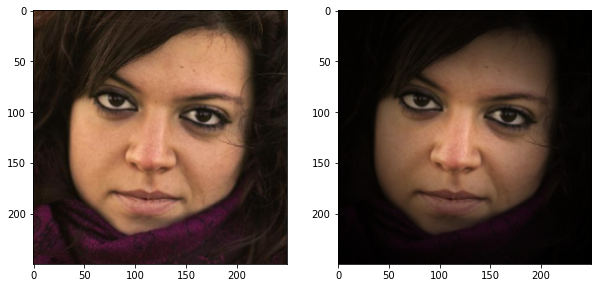
\includegraphics[width=\textwidth]{vignette1}
  \end{subfigure}
  \hfill
  \begin{subfigure}[b]{0.49\textwidth}
    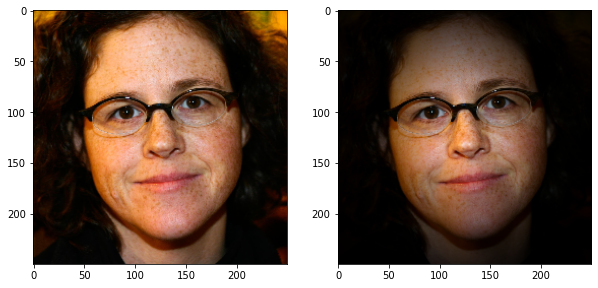
\includegraphics[width=\textwidth]{vignette5}
  \end{subfigure}
  \hfill
  \caption{Vignettes using Gaussian kernels with $\sigma=70$}
  \label{fig:vignette}
\end{figure}

\subparagraph{Cropping} First, I explored the given data set to see where most landmarks are. Then, I thought that some useful information might sit immediately outside of the outer landmarks that might be useful in deciding where the face is (like shadows). Therefore, I cropped the images to remove redundant information (Figure \ref{fig:crop}).

\begin{figure}[h]
  \begin{subfigure}[b]{0.49\textwidth}
    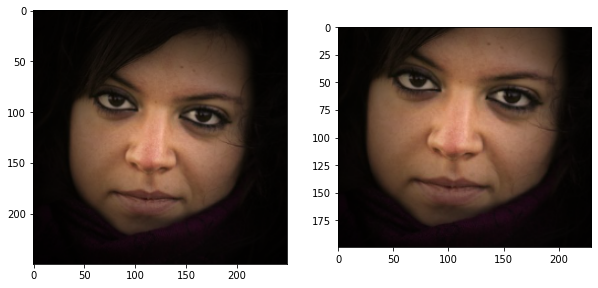
\includegraphics[width=\textwidth]{crop1}
  \end{subfigure}
  \hfill
  \begin{subfigure}[b]{0.49\textwidth}
    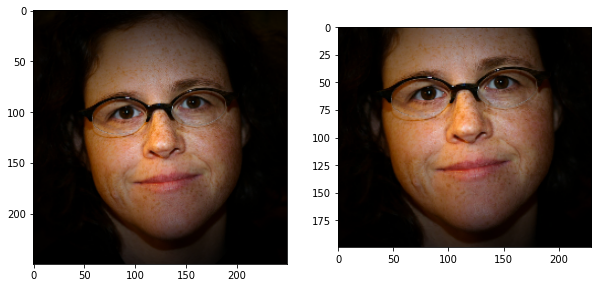
\includegraphics[width=\textwidth]{crop5}
  \end{subfigure}
  \hfill
  \caption{Cropping 40 off the top, 10 off bottom and each of the sides}
  \label{fig:crop}
\end{figure}

\subparagraph{Rescaling} Image features useful for face alignment (e.g. shadows or corners) are still human-discernible in downscaled images. This would reduce training time (Figure \ref{fig:rescale}).

\begin{figure}[h]
  \begin{subfigure}[b]{0.49\textwidth}
    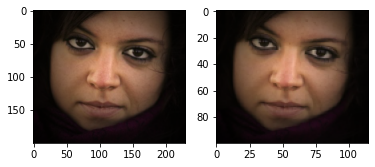
\includegraphics[width=\textwidth]{rescale1}
  \end{subfigure}
  \hfill
  \begin{subfigure}[b]{0.49\textwidth}
    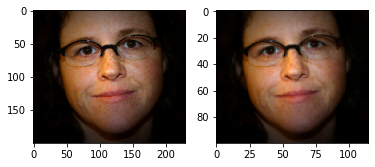
\includegraphics[width=\textwidth]{rescale5}
  \end{subfigure}
  \hfill
  \caption{Rescaling by 50\%}
  \label{fig:rescale}
\end{figure}

\subparagraph{Gaussian Blur} To further reduce the amount of information carried by images, I applied a Gaussian Blur with kernel size $size_{kernel}=(5,5)$ and $\sigma=1$.

\paragraph{Training/Test split}
The training data was randomly split into 80\% training and 20\% test data sets. For the reader to reproduce the results presented in the remainder of the paper, this was done with the \emph{sklearn.model\_selection} method, with $random\_seed$ set to 111.

\subsubsection{Feature extraction}\label{section:feat-extr}
Training a face alignment model using multivariate linear regression requires the same number of features (independent variables) to be extracted from each image. Feature descriptor methods like SIFT and SURF return varying numbers of keypoints between images. HOG, on the other hand, returns the same number of descriptors for each image (given by HOG's parameters like number of orientations and grid size and the image size).

\paragraph{HOG descriptors}
Histogram of Oriented Gradients feature descriptors are usually used in object detection, but here I tried to use it for face alignment. This technique extracts shape and appearance information from pre-set sub-windows of the image in the form of a collection of histograms of intensity gradients or edge directions.

\begin{figure}[h]
  \centering
  \begin{subfigure}[b]{.75\textwidth}
    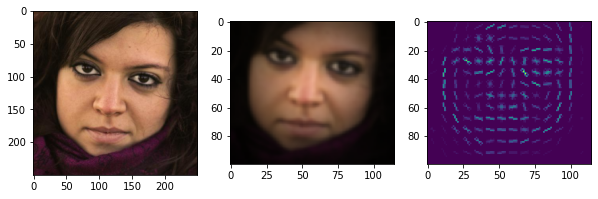
\includegraphics[width=\textwidth]{hog1}
  \end{subfigure}
  \hfill
  \begin{subfigure}[b]{0.75\textwidth}
    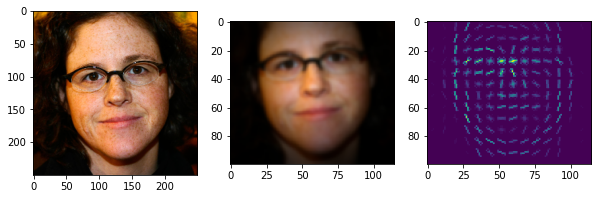
\includegraphics[width=\textwidth]{hog5}
  \end{subfigure}
  \hfill
  \caption{Example HOG feature descriptors (8 orientations, 8x8 pixels per grid cell) from pre-processed images}
  \label{fig:hog}
\end{figure}

\subsubsection{Linear regression}\label{section:linear-reg}
Multivariate linear regression takes a set of observations (or independent variables) $X$, in this case the \textbf{flattened vector of 68 coordinates of face landmarks for each image in the training set}. The model also needs a set of dependent variables $Y$, in this case the \textbf{HOG descriptors} (visualised in Figure \ref{fig:hog}), that the model will learn to predict (linearly fit) given the training landmarks $X$.

To test the accuracy of the model, I extracted the HOG features from the test set images (split in the previous step) and predicted their landmarks. I reshaped the (flat) predictions back into 68 pairs of landmark coordinates.

Thus, the trained model can predict the landmarks of any image given its HOG descriptors, as long as the image has the same size as the training images.

\subsection{Model iterations}

\subsubsection{Average face model}
The simplest model is averaging all the training landmarks into one archetype. This is not very accurate however, given that the current data set has most faces in similar locations and of similar scales, the model \emph{seems} to work.

\begin{figure}[h]
  \centering
  \begin{subfigure}[b]{0.35\textwidth}
    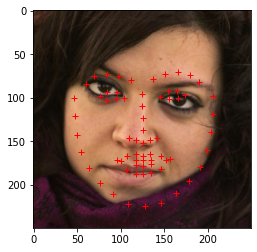
\includegraphics[width=\textwidth]{avg1}
  \end{subfigure}
  \begin{subfigure}[b]{.35\textwidth}
    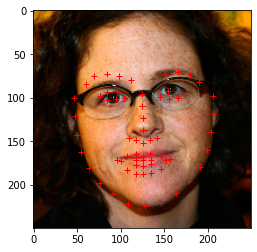
\includegraphics[width=\textwidth]{avg5}
  \end{subfigure}
  \caption{\textbf{\textit{Average face model}} predictions}
  \label{fig:model-avg}
\end{figure}    

\subsubsection{Model A}
\textbf{Data augmentation} (mirroring), \textbf{pre-processing} (vignette, crop, downscale, Gaussian blur), \textbf{HOG} (8 orientations, 8x8 pixels per cell).

Initially I thought that by augmenting (mirroring all training data) and pre-processing the data the model would yield great results, as it would have more data to learn from and would generalise away from unnecessary information (like freckles, stray hairs, etc). However, these led to a very poor performance, especially by predicting stretched or squished face landmarks (see Figure \ref{fig:model-A}).

The model seems to have learned something about rotation and where certain features are (e.g. eyes, eyebrows). I noticed the major irregularities to be on the x-axis and, therefore, assumed mirroring to have been the cause. I investigated this hypothesis next.

\begin{figure}[h]
  \centering
  \begin{subfigure}[b]{0.35\textwidth}
    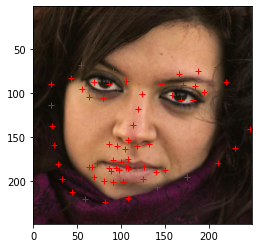
\includegraphics[width=\textwidth]{A1}
  \end{subfigure}
  \begin{subfigure}[b]{.35\textwidth}
    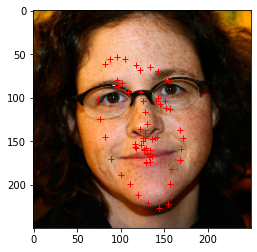
\includegraphics[width=\textwidth]{A5}
  \end{subfigure}
  \caption{\textbf{\textit{Model A}} predictions}
  \label{fig:model-A}
\end{figure}

\subsubsection{Model B}
\textbf{Pre-processing} (vignette, crop, downscale, Gaussian blur), \textbf{HOG} (8 orientations, 8x8 pixels per cell).

As a result of removing augmentation the model gave better results, learning to predict the rotation and outer face landmarks somewhat well.

\textbf{\textit{Model B}}'s weaknesses are picking up fine details (e.g. around the lips) and being more precise about the outer face limit. At this point I thought that I may have gotten rid of too much information such that the HOG descriptors could not pick up fine details that are, in fact, needed for a good prediction.

\begin{figure}[h]
  \centering
  \begin{subfigure}[b]{0.35\textwidth}
    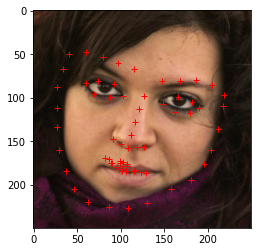
\includegraphics[width=\textwidth]{B1}
  \end{subfigure}
  \begin{subfigure}[b]{.35\textwidth}
    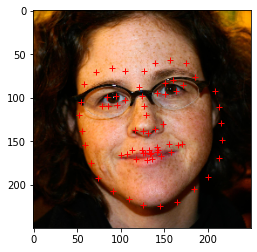
\includegraphics[width=\textwidth]{B5}
  \end{subfigure}
  \caption{\textbf{\textit{Model B}} predictions}
  \label{fig:model-B}
\end{figure}

\subsubsection{Model C}
\textbf{No data augmentation}, \textbf{pre-processing} (vignette, crop, downscale, Gaussian blur), \textbf{HOG} (8 orientations, 4x4 pixels per cell).

Without reducing any of the pre-processing, I just made the HOG descriptors pick up finer information by making the grid cells smaller, from 8x8 to 4x4. Indeed, this taught the model to better predict details around the lips and face edges. However, I was still not satisfied with the accuracy.

\begin{figure}[h]
  \centering
  \begin{subfigure}[b]{0.35\textwidth}
    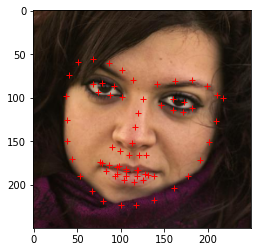
\includegraphics[width=\textwidth]{C1}
  \end{subfigure}
  \begin{subfigure}[b]{.35\textwidth}
    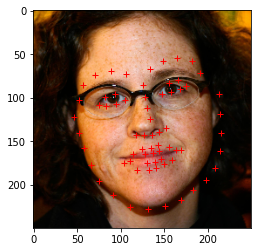
\includegraphics[width=\textwidth]{C5}
  \end{subfigure}
  \caption{\textbf{\textit{Model C}} predictions}
  \label{fig:model-C}
\end{figure}

\subsubsection{Model D}
\textbf{No pre-processing}, \textbf{no pre-processing} \textbf{HOG} (8 orientations, 8x8 pixels/cell).

At this point, after making the HOG descriptors account for finer details, I was curious whether my pre-processing was detrimental to the model learning useful information. I decided to test this hypothesis by fitting the model using HOG descriptors taken from unprocessed images.

I found the results of this model to be satisfactory. Looking at the plotted predictions I felt like they are not too far off from where I would place them. This accuracy would probably work well for simple applications (e.g. simple face filters), while it may not work that well for applications that need very accurate predictions like make-up try-on (e.g. in Figure \ref{fig:model-D}, image on the right, the left eyebrow is predicted to be above where it actually is, potentially resulting in very poor make-up application).

\begin{figure}[h]
  \centering
  \begin{subfigure}[b]{0.35\textwidth}
    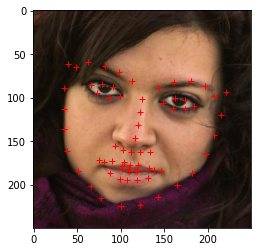
\includegraphics[width=\textwidth]{D1}
  \end{subfigure}
  \begin{subfigure}[b]{.35\textwidth}
    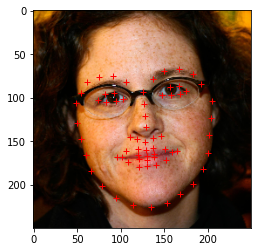
\includegraphics[width=\textwidth]{D5}
  \end{subfigure}
  \caption{\textbf{\textit{Model D}} predictions}
  \label{fig:model-D}
\end{figure}

\subsection{Model analysis}
The accuracy of a model is calculated as the average Euclidean distance from the predicted landmarks to the true landmarks of the test set (split before training).

The cumulative density measure shows a steady increase in accuracy performance over the model iterations (Figure \ref{fig:avgBCD}). \textbf{\textit{Model A}}, lower in performance than \textbf{\textit{Model B}} but higher than the \textbf{\textit{Average face model}} was left out for legibility (its performance being calculated on double the test data due to augmentation).

\begin{figure}[h]
  \centering
  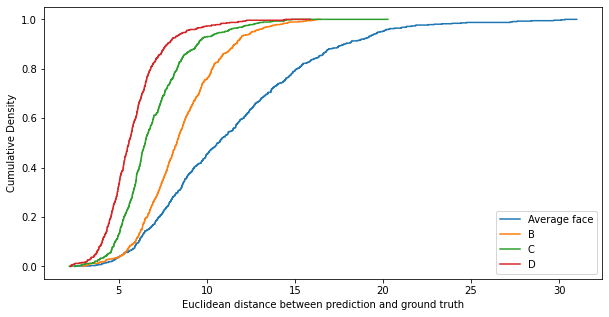
\includegraphics[width=.8\textwidth]{avgBCD}
  \caption{Cumulative density measures of discussed models (except \textbf{\textit{Model A}})}
  \label{fig:avgBCD}
\end{figure}

\begin{figure}[h]
  \centering
  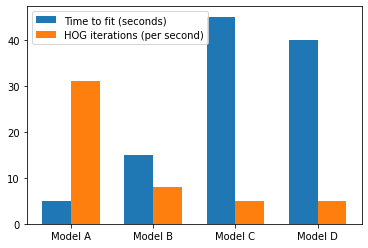
\includegraphics[width=.5\textwidth]{ABCD}
  \caption{Training time performance comparison}
  \label{fig:ABCD}
\end{figure}

\subsection{Discussion}

\subsubsection{Pre-processing}
One of the main lessons for me was that I should first try and extract features from the raw data, without any pre-processing, instead of blindly pre-processing images based on a priori assumptions. In this case, pre-processing decreased the average model accuracy.

\subsubsection{Training time bottleneck}
As seen in Figure \ref{fig:ABCD}, the higher the data dimension (image size, scale), the longer it takes to compute the HOG descriptors. Computing HOG descriptors is the clear time bottleneck of training and testing. For some applications (high frames-per-second video face alignment), fast descriptor computation is key, so a trade-off with accuracy might be needed.

\subsubsection{Potential improvements}
I am very surprised by \textbf{\textit{Model D}}'s accuracy, given its very simple architecture. However, there are many areas of improvement (e.g. details around the eyebrows, eyes or lips). Learning high-level information (roll, yaw, pitch) and low-level information (smile, open mouth) all at the same time might be too demanding from one linear regression model.

One possibility of improvement is having a cascade of linear regression models, with early models learning high-level information and later models dealing with fine adjustments.

\section{Pixel segmentation}

\begin{figure}[h]
  \centering
  \begin{subfigure}[b]{.75\textwidth}
    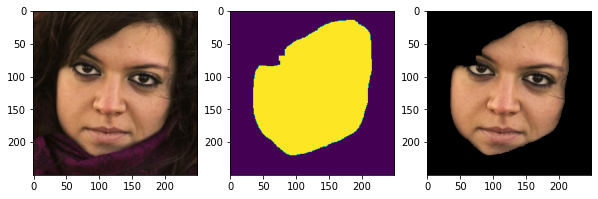
\includegraphics[width=\textwidth]{seg1}
  \end{subfigure}
  \hfill
  \begin{subfigure}[b]{0.75\textwidth}
    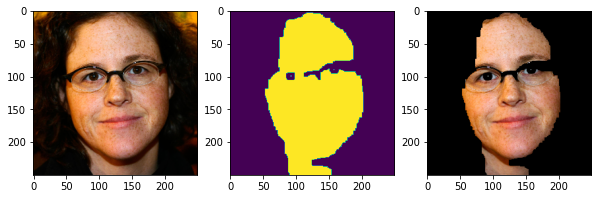
\includegraphics[width=\textwidth]{seg5}
  \end{subfigure}
  \hfill
  \caption{Pixel segmentation using GrabCut (original image, 5th iteration, face pixels extracted}
  \label{fig:sig}
\end{figure}

A potential improvement for the GrabCut method to include all pixels within the boundary defined by the predicted landmarks.

\section{Face effects}

Inspired by Canu \cite{canu_2019}, I have created a Clown Nose face filter. The red nose dynamically scales according to the scale of the face (landmarks). Potential improvements include brightness and contrast matching (to the source image) and 3D perspective alterations using the face landmarks.

\begin{figure}[h]
  \centering
  \begin{subfigure}[b]{.4\textwidth}
    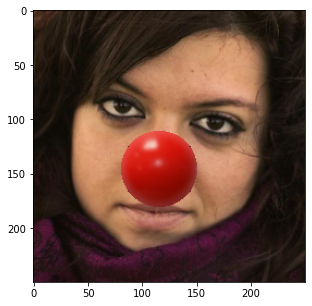
\includegraphics[width=\textwidth]{nose1}
  \end{subfigure}
  \begin{subfigure}[b]{0.4\textwidth}
    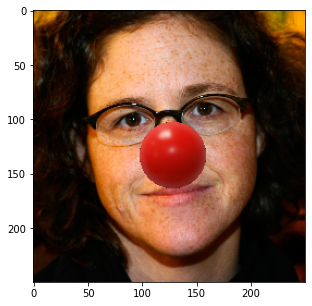
\includegraphics[width=\textwidth]{nose5}
  \end{subfigure}
  \caption{Clown Nose filter}
  \label{fig:nose}
\end{figure}

\newpage
\bibliographystyle{plain}
\bibliography{bibliography.bib}

\end{document}